\ofjob{Bard}
{
	\ofquote{"Welcome to your doom, starring me!"\\}{Rikku}\\\\
	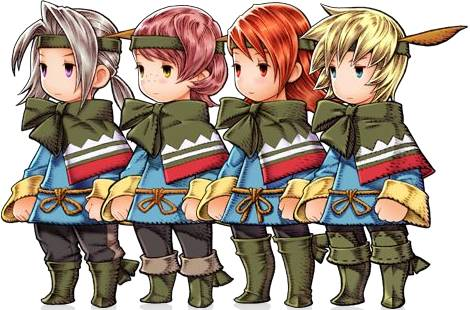
\includegraphics[width=\columnwidth]{./art/jobs/bard.jpg}\ofrow
	\accf{Bards} blur the lines between art and war.
	They can perform songs and dances that bestow powerful benefits for allies and vicious handicaps for enemies.
	Even though Bards are not the most powerful duelists, they can often turn the tide of a battle in unexpected ways.
}
{Dagger}{Light Armor or Robe}{
	Level 1: & HP~+19 & MP~+20 & AGI~+3 & RES~+1  \\
	Level 2: & HP~+10  & MP~+10 & DEF~+1  \\
	Level 3: & \multicolumn{3}{l}{Archetype Attribute Bonus} \\
	Level 4: & HP~+5  & MP~+10 & RES~+1 & DEF~+1 \\
	Level 5: & HP~+10 & MP~+5  & STR~+2 \\ 
	Level 6: & HP~+5  & MP~+10 & RES~+1 & DEF~+1 \\
	Level 7: & HP~+10 & MP~+10 & STR~+1 &  	  \\
	Level 8: & HP~+10  & MP~+10 & DEF~+1 \\
	Level 9: & HP~+10 & MP~+10 & STR~+1 \\
	Level 10: & HP~+5  & MP~+10 & RES~+1 & DEF~+1	
}{
	\ofjobtech{Cheer}{5}{0r}{1u}{Self}{Everyone in the target area can choose to either gain \mbox{EnSTR} or EnMAG for 2 rounds.}{\enstr\enmag}{1}\ofabilitygap
	\ofjobtech{Improvise}{6}{0r}{Single}{5u}{Roll 1d. Based on the result, the target gains the following Status Effect for 3 rounds:\\ 1-EnDEF, 2-EnRES, 3-EnSTR, 4-Blink, 5-Regen, 6-Haste.}{}{2}\ofabilitygap
	\ofjobtech{Spotlight}{8}{0r}{2u}{Self}{You create an Obscure Field around yourself that follows you for 3 rounds, but does not affect you.}{}{4}\ofabilitygap
	\ofjobtech{Mighty March}{12}{0r}{2u}{Self}{You and all allies in the target area gain Haste and EnDEF for 2 rounds.}{\enndef\enres}{6}\ofabilitygap
	\ofjobtech{Charm}{14}{1r}{Single}{4u}{Choose an enemy as the target. He makes a DC~8 check and upon failure he immediately takes an extra turn following your command. The turn order is unchanged. Some enemies may be Immune to this effect.}{}{8}\ofabilitygap
	\ofjobtech{Mimic}{?}{0r}{?}{?}{You use an ability that was used by an ally or enemy on the battlefield since your last turn. In doing this, you have to respect the MP cost, cast time as well as the target and range specifications of the copied ability.}{}{10}
}{
	\ofarchetypet{Dancer}
	{HP~+12 & MP~+8 & STR~+2 & DEF~+1}
	{\ofarchetypetecha{Blade Dance}{6}{0r}{Single}{Weapon}{Make an Attack on the target. Then you can immediately choose another target within 2u, dash towards him and make an Attack on him as well.}{}}
	{\ofspecial{Dress to Impress}{You can equip one additional Accessory. Also, as long as you have at least 2 Accessories equipped, you additionally gain DEF +1 and RES +1.}{5}{\oficonpassive}}	
	{\ofspecial{Dirty Dancing}{Whenever you successfully evade an Attack, you can immediately inflict one of the following Status Effects on the attacker for 3 rounds: Immobile, Poison, Blind.}{7}{\oficonreaction}}
	{\ofarchetypetechb{Slow Dance}{12}{0r}{2u}{Self}{You create a special Field around yourself that lasts for 3 rounds and simultaneously acts as a Slow Field, Hot Field and Slippery Field. The Field moves together with you and it only affects enemies.}{}}
}{
	\ofarchetypet{Singer}
	{HP~+4 & MP~+16 & RES~+3}
	{\ofarchetypetecha{Requiem}{8}{0r}{Single}{4u}{The target makes a DC~8 check and upon failure he suffers dark damage equal to two times your current Level and Zombie for 3 rounds.}{\zombie\dark}}
	{\ofarchetypepassive{Encore}{Whenever you bestow one or more positive Status Effects on a target, additionally restore his HP by an amount equal to your current Level.}}
	{\ofarchetypereaction{Duet}{Whenever an ally within 1u of you performs an Attack or uses an ability on an enemy, you can immediately use an ability either on your ally or on the affected target if he is within range.}}
	{\ofarchetypetechb{Lullaby}{12}{0r}{3u}{5u}{All enemies in the target area make a DC~8 check and suffer 3d damage and Sleep for 3 rounds upon failure.}{\sleep}}
}